\documentclass[generalized_symmetry.tex]{subfiles}
\setcounter{chapter}{1}
\begin{document}
\chapter{対称性とトポロジカル欠陥}\label{sec:symmetrydefect}

この章の目標は、前章で紹介した対称性の③の見方「対称性とは余次元1のトポロジカル欠陥で群構造を持つもの」ということを納得してもらうことです。まず、欠陥という概念を導入します。そして対称性がトポロジカル欠陥であることを様々な観点から説明します。一旦それを納得してもらえば、対称性の一般化はすんなりと納得してもらえると思います。

\section{欠陥}\label{sec:defect}

まず、欠陥を定義します。
\begin{emphasize}
  場の理論において\kyou{欠陥(defect)}とは、\kyou{時空の中で他の部分と性質が異なる部分}のことを言います。 ただし、局所性を満たすものとします。 
\end{emphasize}

補足の説明をします。性質が異なるというのは、例えばLagrangian密度がそこだけ異なるとか、余分な自由度がそこにあるとか、格子の理論なら、そこだけ格子の構造が異なるとか、そういうものです。

局所性というのは、性質が異なるとしても非局所的な相互作用はないということです。言い換えれば、欠陥の上の離れた2点が直接相互作用をすることは無いようなものです。格子理論で考える場合には、連続極限をとったときに局所性を満たすようなものなら、それは局所性を満たす欠陥であると言うことにします。

別の言い方をすると、欠陥とは(広い意味での)演算子であるということもできます。

次に2つの言葉を導入します。まず、欠陥の\kyou{次元}とは、性質の異なる部分の次元を言います。例えば時空の中で1点が他の部分と異なるなら、その次元は1です。\kyou{余次元(codimension)}とは、時空の次元を$d$、欠陥の次元を$p$としたときに、$d-p$のことを言います。欠陥の性質は余次元によって共通な場合もあるので、この言葉を導入するのが便利です。これは単に言葉遣いの問題なのですが、余次元0の欠陥、つまりある領域にわたって性質が違うようなものは欠陥とは呼ばないことにします。

代表的な欠陥の例を2つ挙げます。局所演算子は0次元の欠陥です。別の言い方をするなら、局所演算子とは時空の1点にある欠陥の別名です。\footnote{局所演算子はLagrangianに出てくる場の微分やそれらの積で書けているものに限りません。}もう一つの例はゲージ理論のWilsonループ$\Tr P \exp\left(i\oint A\right)$です。Wilsonループは1次元の欠陥の例です。

欠陥について一つ注意することは、欠陥は動的な物体、例えばソリトンなどではないということです。動的な物体は運動方程式などにしたがって運動しますが、欠陥はその部分の物理法則を手で変えるようなものです。欠陥の形などは手で決めます。ややこしいことに文献によってはソリトンのことを欠陥と呼んでいるものもあるので注意が必要です。

\section{対称性とトポロジカル欠陥その1}

ここから対称性とトポロジカル欠陥の関係について見ていきます。

まず、\kyou{トポロジカル欠陥(topological defect)}とは、欠陥のうちでトポロジーを変えない連続変形で値を変えないもののことを言います。\footnote{これも不幸な用語の行き違いなのですが、トポロジー的に守られて安定なソリトンのことをトポロジカル欠陥と呼ぶ文献もあります。これはこの講義でのトポロジカル欠陥とは違うものです。}
絵を使った式で書くなら
\begin{align}
  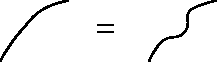
\includegraphics{topologicaldefect.pdf}
\end{align}
のようになります。この式も\ref{sec:remarks}節で述べた演算子関係式の書き方を使っています。つまり、左辺と右辺は他に任意の共通の演算子が挿入されている期待値です。ただし、欠陥を変形している部分には演算子は挿入されていません。

ここから考えていきたいことは、みなさんが納得しているはずの対称性の見方②$\Hh \Uh = \Uh \Hh$、および④$\del_{\mu}J^{\mu}=0$から始めて、③トポロジカル欠陥の見方ができることを示すことです。

\subsection{ユニタリー演算子とトポロジカル欠陥}

$d$次元の場の理論の演算子形式の定式化から始めることにします。簡単のために$\U (1)$対称性の場合を考えます。時刻$0$で対称性のユニタリー演算子は変換のパラメーターを$\alpha$として、
\begin{align}
  \Uh=e^{i\alpha \Qh},\qquad
  \Qh:=\int_{t=0,\ \text{空間}}d^{d-1}x \Jh^0. 
\end{align}
$\Jh^{0}$はカレント$\Jh^{\mu},\ \mu=0,\dots,d-1$の時間方向成分、つまり電荷密度です。$\Qh$の定義は空間が有限(周期境界条件など)の場合には良いですが、無限の場合には積分が定義されるかどうかが問題となります。実は自発的対称性の破れが起こっている場合には、この積分は収束しません。自発的対称性の破れについては、教科書\cite{Kugo2}が詳しいです。ここではひとまず定義されている場合を考えることにします。

Euclideanの定式化を使うために、
\begin{align}
  \Jh^{d}:=i\Jh^{0}
\end{align}
を定義します。\footnote{これを見て分かるように、Euclideanの定式化ではHermit共役には注意する必要があります。} これを用いると
\begin{align}
  \Qh = -i \int_{t=0,\ \text{空間}}d^{d-1}x \Jh^{d}
\end{align}
と書けます。

Euclid時間(虚時間)を$\tau$として、Euclid時間発展について考えます。$\Oh$を時刻$0$での演算子として、Heisenberg演算子のような役割をする演算子$\Oh(\tau)$を
\begin{align}
  \Oh(\tau):=e^{\tau \Hh}\Oh e^{-\tau \Hh}
\end{align}
と定義します。\footnote{本当のHeisenberg演算子と区別するために記号を変える方が良いのかもしれませんが、煩雑になるのでやめておきます。本物のHeisenberg演算子とは違うものであることに注意してください。また、ここで定義したEuclideanのHeisenberg演算子のようなものは取り扱いには注意が必要です。$e^{|\tau| \Hh}$という高エネルギーのところが大きく効いてくる演算子が入っているからです。ただし、これらの演算子の時間順序積の真空期待値などはちゃんと定義されます。Euclideanの経路積分形式と演算子形式をつなぐときに考えると便利な書き方だと思うと良いと思います。} こうすると、例えばカレントの保存則$\del_{\mu}\Jh^{\mu}(x^0,\vec{x})=0,\ \mu=0,\dots, d-1$は、$x^d:=\tau$として
\begin{align}
  \del_{\mu}\Jh^{\mu}(\vec{x},x^{d})=0,\ \mu=1,\dots,d
\end{align}
と書くことができます。また、$\Uh \Hh = \Hh \Uh$ですから
\begin{align}
  \Uh(\tau)=\Uh
  \label{conservation}
\end{align}
となります。

式\eqref{conservation}をEuclidean経路積分形式での期待値の関係式に書くと
\begin{align}
  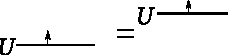
\includegraphics{conservation.pdf}\label{coservationfig}
\end{align}
のようになります。ここで矢印で向きを表しています。

$U$は時間一定面で他の部分とは異なっているので、余次元1の欠陥です。式\eqref{coservationfig}は、$U$を時間方向にずらしても値を変えないことを示しています。これから、$U$がトポロジカル欠陥であることを示します。

これから書くのはEuclidean経路積分形式での演算子関係式です。余次元1の向きのついた部分多様体を$M$として
\begin{align}
  U(M):=e^{i\alpha Q(M)},\quad
  Q(M):=-i\int_{M}dS_{\mu}J^{\mu}
\end{align}
とします。\footnote{$U(M)$の定義の中に$\exp$があって、同じ点での演算子の積が入っています。一般には、ここで発散があったり、繰り込みが必要だったりして微妙なことが起こるのですが、ここではひとまず説明のために無視します。正しい取り扱いは、次節でやる背景ゲージ場とそのゲージ変換を用いる方法です。}$\int_{M}dS_{\mu}$は電磁気の授業などで出てきた面積分です。

この$U(M)$がトポロジカルであることは次のようにして示します。ある領域$D$があって、$\del D=M\cup (-M')$とします。ただし、$-M'$は$M'$の向きを反対にしたものです。こうするとGaussの定理を用いて
\begin{align}
  \int_{D}d^d x \del_{\mu}J^{\mu}
  =\int_{M}dS_{\mu}J^{\mu}-\int_{M'}dS_{\mu}J^{\mu}
\end{align}
を得ます。ここから
\begin{align}
  Q(M)=Q(M'),\qquad U(M)=U(M')
\end{align}
という式が成り立ちます。特に$M_1$と$M_2$がトポロジーを変えない連続変形で繋がっている場合には領域$D$で、$\del D=M_1\cup (-M_2)$となるものがとれますから、$U(M_1)=U(M_2)$となり、したがって$U$はトポロジカル欠陥ということが言えました。

ここまでで言えたことをまとめます。
\begin{emphasize}
  対称性があると対応するトポロジカル欠陥がある。それは、対称性の演算子$\Uh$を時間一定面だけでなく、曲がったところにも定義したものである。
\end{emphasize}
最初の方で、自発的対称性の破れがあるときには$\Uh$がうまく定義できないと言いました。しかし、これは定義しようとしている空間が無限であるところからくるものです。したがって、$M$が有限である場合には$U(M)$は自発的対称性の破れがあるかどうかにかかわらず定義でき、理論の解析に用いることができます。

\subsection{局所演算子への作用}

次に対称性の局所演算子への作用について考えてみます。場の理論の演算子形式では、局所演算子$\Oh(x)$変換は
\begin{align}
  \Uh \Oh(x) \Uh^{\dag}=\Oh'(x)
  \label{transformation0}
\end{align}
と書けます。\footnote{量子力学の教科書とは異なるconventionを用いています。場の理論の論文では、ここで用いるconventionの方が一般的です。}
$\Uh,\Uh^{\dag}$は$\Hh$と可換ですから、$\Uh$を少しだけ虚時間で未来に移動し、$\Uh^{\dag}$を少しだけ過去に移動することで
\begin{align}
  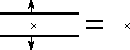
\includegraphics{transformation0.pdf}
\end{align}
という絵で表すことができます。別の言い方をすると式\eqref{transformation0}の左辺は、
\begin{align}
  T(\Uh(M_1)\Oh(x)\Uh(M_2))=T(\Uh(M)\Oh(x)),\quad
  M:=M_1 \cup (-M_2)
\end{align}
と表すことができます。$T()$は虚時間順序積を表します。さらに$\cdots$を$x$と同時刻にはない任意の演算子の挿入として\eqref{transformation0}より
\begin{align}
  \ev{T(\Uh(M)\Oh(x)\cdots)}{0}=\ev{T(\Oh'(x)\cdots)}{0}
\end{align}
という式が成り立ちます。この両辺に現れる量をEuclidean経路積分で表すことを想定して
\begin{align}
  \expval{U(M)\Ocal(x)\cdots}=\expval{\Ocal'(x)\cdots}
\end{align}
と書くのでした。さらにこれを略記して
\begin{align}
  U(M)\Ocal(x) = \Ocal'(x)
\end{align}
と書きます。$U(M)$はトポロジカルですから、連続変形して(変形後の面も同じ記号$M$で表すことにして)
\begin{align}
  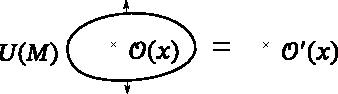
\includegraphics{transformation1.pdf}
\end{align}
という絵で書きます。これが、局所演算子の変換性をトポロジカル欠陥を用いて表したものになります。後で示すように、これはWard-Takahashi恒等式を有限変換の場合にも適用できる形にしたものと言うこともできます。

\section{対称性とトポロジカル欠陥その2}
ここでは、対称性とトポロジカル欠陥の関係を先程とは少し別の角度から見てみます。ここでは、通常のWard-Takahashi恒等式を①の描像から導くのと同様の方法を離散対称性の場合にも適用できるように有限変換で行います。つまり、大域的対称性であっても場所に依存する変換し、それによる作用の変化を見ます。

\subsection{分配関数と対称性欠陥}
$d$次元の場の理論を考えます。場を$\phi(x)$とし、作用を$S(\phi)$とします。この系に①の意味での大域的対称性があるとします。つまり、群$G$があり、$g\in G$に対して変換$\phi(x) \to \phi^g(x)$があって、$S(\phi^g)=S(\phi)$となるとします。$G$は連続的でも離散的でも良いです。

アイデアは、大域的対称性であっても場所に依存する変換、つまりゲージ変換をしてみることです。離散対称性でも適用できるように次のような変換を考えます。Euclidean時空の中の領域$D$をとり、変換
\begin{align}
  \phi'(x)=
  \begin{cases}
    \phi^g(x), & x\in D\\
    \phi(x), & x \notin D
  \end{cases}
  .\label{gaugetransf}
\end{align}
を考えます。つまり、領域$D$内では、$g$での変換を行い、$D$の外では変換しません。この変換を用いて分配関数を変形していきます。
\begin{align}
  Z&=\int D\phi e^{-S(\phi)}\notag\\
   &= \int D\phi' e^{-S(\phi')}\notag\\ 
   &= \int D\phi e^{-S_{D,g}(\phi)}.\label{derWT1}
\end{align}
この変形では、1行目から2行目は単に積分変数の文字を変えただけです。2行目から3行目へは変換\eqref{gaugetransf}を代入しました。簡単のため、この変換で積分測度$\int D\phi$は不変であることを仮定しました。また、$S_{D,g}(\phi):=S(\phi')$と定義しました。

さて、一般には変換で$S_{D,g}(\phi)\ne S(\phi)$です。どれくらい異なるかを考えてみましょう。まず、$D$の外部では$\phi(x)=\phi'(x)$ですから、同じです。一方、$D$の内部では$\phi\to \phi^g$が大域的対称性であることから、同じになることが分かります。つまり、\kyou{$S_{D,g}(\phi)$と$S(\phi)$は$M:=\del D$の部分でのみ異なることになります。} ですので、$M$に局在している演算子(欠陥)を
\begin{align}
  U_{g^{-1}}(M):=\exp(S(\phi)-S_{D,g}(\phi))
\end{align}
の挿入で定義することにします。すると\eqref{derWT1}から
\begin{align}
  Z=\int D\phi e^{-S(\phi)}U_{g^{-1}}(M)
\end{align}
を得ます。この両辺を$Z$で割ると
\begin{align}
  \expval{U_{g^{-1}}(M)}=1
\end{align}
という恒等式を得ます。これがWard-Takahashi恒等式の一種です。

$D$の外側に他の演算子(欠陥)がささっている場合も全く同様の変形ができて、次の恒等式を得ます。
\begin{align}
  \expval{U_{g^{-1}}(M)\cdots}=\expval{\cdots}
\end{align}
このような式を単に
\begin{align}
  U_{g^{-1}}(M)=1\quad (\text{ただし$M$の内側には他の演算子がささっていない})
\end{align}
と式で表したり、
\begin{align}
  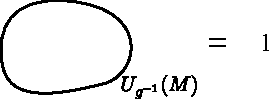
\includegraphics{EgWTid0.pdf}
\end{align}
と絵で表したりするのでした。

\subsection{演算子への作用}
この見方で演算子への作用を考えてみます。$\Ocal(x)$を局所演算子とし、それが$g\in G$で$\Ocal^{g}(x)$と変換するとします。

$D$の内部に$\Ocal(x)$を置き、その他の任意の演算子(欠陥)を$D$の外部に置きます。そして先程と同じように\eqref{gaugetransf}を考えます。すると
\begin{align}
  Z\expval{\Ocal(x)\cdots}
  =\int D\phi \Ocal(x)\cdots e^{-S(\phi)}
  =\int D\phi U_{g^{-1}}(M)\Ocal^{g}(x)\cdots e^{-S(\phi)}
\end{align}
という恒等式を得ます。これは
\begin{align}
  U_{g^{-1}}(M)\Ocal^{g}(x)=\Ocal(x)
\end{align}
と書くのでした。ここで、$\Ocal^{g}(x)$のことを$\Ocal(x)$と書き$g$のことを$g^{-1}$と書くことで
\begin{align}
  U_{g}(M)\Ocal(x)=\Ocal^{g}(x)
\end{align}
という恒等式を得ます。これは絵で
\begin{align}
  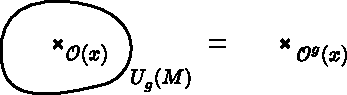
\includegraphics{EgWTid1.pdf}
\end{align}
というふうに表すこともできます。

$G$は群ですから、演算子への作用も表現になっています。ですから、表現行列を用いてWard-Takahashi恒等式を表しておくことも便利です。すべての局所演算子の基底を$\Ocal_{a}(x)$とすると、$\Ocal_{a}^{g}(x)$はこれらの線形結合で表すことができます。つまり$R(g)^{b}{}_{a}$を表現行列として
\begin{align}
  \Ocal^{g}_{a}(x)=\sum_{b}\Ocal_{b}(x)R(g)^{b}{}_{a}
\end{align}
と書くことができます。
これらすべてまとめて次のように言うことができます。
\begin{emphasize}
  離散的な群の場合も含めて、トポロジカル欠陥が対称性の局所的な記述を与える。この対称性を記述するトポロジカル欠陥を\kyou{対称性欠陥}と呼ぶ。Ward-Takahashi恒等式は
  \begin{align}
    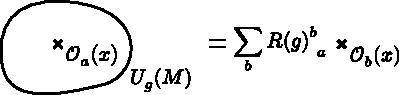
\includegraphics{EgWTid2.pdf}
  \end{align}
  と表せる。    
\end{emphasize}

\subsection{背景ゲージ場}\label{sec:backgroundgaugefield}
対称性を表すトポロジカル欠陥の便利な見方の一つは、背景ゲージ場を考えることです。結論から言うと、flatな背景ゲージ場の背景が対称性のトポロジカル欠陥の配位と同一視できます。それをこれから説明していきます。

簡単のため、連続対称性でアノマリーが無い場合を考えます。前節と同じ設定で、大域的対称性の背景ゲージ場$A$を入れた作用を$S(\phi,A)$とします。$A=0$のときに元の作用に戻るとします。つまり$S(\phi,A=0)=S(\phi)$とします。この背景ゲージ場の元での分配関数は
\begin{align}
  Z(A)=\int D\phi e^{-S(\phi,A)}
\end{align}
と表すことができます。

ここでゲージ変換について考えてみます。$A=0$のところから、前項で考えたゲージ変換\eqref{gaugetransf}をしてみます。このとき、$A\to A'$と変化します。ゲージ不変性は仮定しているので
\begin{align}
  Z(A=0)=Z(A')
\end{align}
となります。前項で議論したように、左辺は$M=\del D$に対称性欠陥が入った分配関数です。これがゲージ場$A'$が入っているのと同じということです。

$A'$は$A=0$から\eqref{gaugetransf}から得られたものですから、$A'$は$M$上だけでデルタ関数的に非0の値を持っています(図\ref{fig:localizedgaugefield}参照)。その値は$D$の中の点から外の点への経路で$M$と1回交わる経路を$C$として
\begin{align}
  P e^{i\int_{C}A'} = g
\end{align}
となるようになっています。また、もともと場の強さは$0$でしたから、ゲージ変換した後も$0$となります。このように場の強さが0となるゲージ場の配位を\kyou{flat}なゲージ場といいます。

\begin{figure}
  \centering
  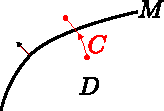
\includegraphics[width=6cm]{localizedgaugefield.pdf}
  \caption{対称性欠陥と背景ゲージ場の配位。$M$上にある対称性欠陥は$M$上にデルタ関数的に局在した背景ゲージ場の配位として表すことができる。$P e^{i\int_{C}A'} = g$ となるようになっている。}
  \label{fig:localizedgaugefield}
\end{figure}

この結果をまとめると
\begin{emphasize}
  対称性欠陥は、デルタ関数的に局在した背景ゲージ場の配位である。
\end{emphasize}
と言えます。

この逆を考えてみましょう。flatな背景ゲージ場の配位が与えられたとします。するとある点のまわりの球体のトポロジーを持つ領域でゲージ変換して、$A=0$とすることができます。これを図\ref{fig:localizedgaugefield}のように空間のいろんな部分からやっていって、ほとんどの部分で$A=0$とすることができます。しかし、二人の人が別の点からゲージ変換していって、ぶつかったときに、その間ですべて$A=0$とすることができるとは限りません。一般に2つの領域の境目で$A\ne 0$となります。言い換えると、2つの領域の境目が対称性欠陥となります。

\begin{figure}
  \centering
  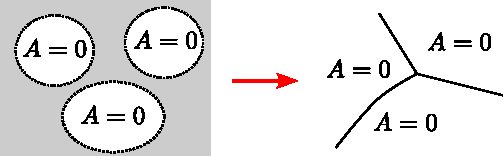
\includegraphics{flatgaugefield.pdf}
  \caption{flatな背景ゲージ場の配位と対称性欠陥の関係。右のようにいろんな点のまわりの球体の領域でゲージ変換を行って$A=0$となるようにする。領域の境目のみで$A\ne 0$になるが、これが対称性欠陥になる。}
  \label{fig:flatgaugefield}
\end{figure}

図\ref{fig:flatgaugefield}を見てもらっても分かるように、この操作を行うと一般的に対称性欠陥が枝分かれしている\kyou{ジャンクション}ができます。ゲージ変換によってジャンクションも連続的に動かすことができるので、このジャンクションもトポロジカルです。このジャンクションで繋がれるトポロジカル欠陥は何でもよいわけではなく、flatであることからジャンクションまわりのWilsonループが1になるので、それぞれの欠陥に割り振られる群の元は
\begin{align}
  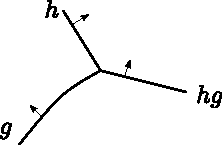
\includegraphics{junction.pdf}
\end{align}
という関係になります。

図\ref{fig:flatgaugefield}では2次元的に書いているので余次元2のジャンクションだけですが、高次元ではこのようなジャンクションがさらに集まったジャンクションもできます。3次元空間の中で泡が集まっているようなものを思い浮かべてください。

まとめると
\begin{emphasize}
  flatなゲージ場の配位は、様々な次元のトポロジカルなジャンクションを含む対称性欠陥の配位で表される。
\end{emphasize}

一般のこのような対称性欠陥の配位の元での分配関数は理論の詳細によります。しかし、対称性のみから導かれるWard-Takahashi恒等式から分かる部分もあります。

\subsection{Ising模型のspin flipの例}\label{sec:egspinflip}
前項までは、連続的な場の理論の描像で対称性がトポロジカル欠陥で表されることを見てきました。連続的な場合には正則化など場の理論特有の微妙な問題もあって、数学的に厳密な取り扱いが難しいです。この項では、格子上でのIsing模型のspin flipの対称性を例にとって、対称性とトポロジカル欠陥を考えてみます。この場合には、経路積分が有限和になりますから、数学的に厳密な取り扱いが可能となります。

まず、Ising模型を定義します。$d$次元の立方格子を考えます。周期境界条件を課して有限個のサイトがあるような場合を考えます。サイトのラベルを$i,j,\dots$とします。各サイト$i$に自由度$a_i=0,1$を置きます。そして$K$を正の実数として、分配関数をすべての$a_i=0,1$の足し上げ
\begin{align}
  Z:=\sum_{\{a\}}e^{-S(a)},\quad
  S(a):=-K \sum_{\link{ij}:\text{すべてのリンク}}(-1)^{a_i+a_j}
  \label{ddimIsing}
\end{align}
で定義します。ここでサイト$i,j$をつなぐリンクを$\link{ij}$で表しました。これは有限和ですから、数学的に厳密な取り扱いができます。\footnote{ここで数学的に厳密に取り扱いを説明するという意味ではありません。}

このIsing模型にはspin flipの対称性
\begin{align}
  a_i \to a_i+1 \mod{2}
\end{align}
があります。この対称性を表すトポロジカル欠陥がどのようなものかを考えてみましょう。そのために領域(サイトの集合)$D$をとり、変換
\begin{align}
  a'_i=
  \begin{cases}
    a_i+1,& i\in D\\
    a_i,& i \notin D
  \end{cases}
  \label{gaugespinflip}
\end{align}
を考えます。ここで、\eqref{ddimIsing}の分配関数は
\begin{align}
  Z=\sum_{\{a\}}e^{-S(a)}=\sum_{\{a'\}}e^{-S(a')}=\sum_{\{a\}}e^{-S_{D}(a)}
\end{align}
と変形できます。最初は和を取っている変数の文字を変えただけです。次は\eqref{gaugespinflip}を代入し、明らかに成り立つ性質$\sum_{\{a'\}}=\sum_{\{a\}}$を用いました。また、$S_{D}(a):=S(a')$を定義しました。

$S_{D}(a)$と$S(a)$の違いを見てみましょう。リンク$\link{ij}$に関して、$i,j\notin D$の場合には変換しないので変化なし、$i,j\in D$の場合にも両方のスピンが反転するので、相互作用は変化しません。変化するのは片方が$D$に入っていて、もう片方は$D$に入っていない場合、つまりリンクが$D$の境界にある場合です。このようなリンクは、分配関数への寄与が
\begin{align}
  \exp\left(-K(-1)^{a_i+a_j}\right)
\end{align}
と反強磁性の相互作用になります。したがって$M=\del D$の部分でのみ相互作用が反強磁性になっていて、他の部分と異なっています。したがって、これは余次元1の欠陥になります。また、いろんな領域をとって\eqref{gaugespinflip}の変換をすることによって、分配関数の値を変えずに連続的に\footnote{格子理論で「連続的」は奇妙な感じがしますが、ここでは、境界付近にあるサイト一つだけまたぐ変形を繰り返してできる変形を「連続的な変形」と呼んでいます。}欠陥を動かすことができるので、この欠陥はトポロジカルです。つまり、この欠陥が対称性を表すトポロジカル欠陥である「対称性欠陥」です。

このspin flipのトポロジカル欠陥とゲージ場の配位の関係についても見ておきましょう。先程出てきた$S_{D}$は次のように書くことができます。
\begin{align}
  S_{D}(a):=-K\sum_{\link{ij}}(-1)^{a_i+a_j+b_{ij}},\quad
  b_{ij}=\begin{cases}
    0, & \link{ij}\notin M\\
    1, & \link{ij} \in M
  \end{cases}.
\end{align}
この$b_{ij}$は、リンクに群$\Zb_2$の元$0,1$が配置されているので、格子理論における$\Zb_2$背景ゲージ場と思うことができます。
格子ゲージ理論については、後ほど詳しく説明します。このゲージ場の配位$b_{ij}$は次のようにflatという性質を満たします。格子においてサイトを頂点とする最小の正方形をプラケット(plaquette)と呼ぶことにします。任意のプラケットをとってきて、それを囲む4つのリンクを$\link{ij},\link{jk},\link{kl},\link{li}$とします。このとき上の$b$は
\begin{align}
  b_{ij}+b_{jk}+b_{kl}+b_{li}=0 \mod{2}
\end{align}
を満たします。このようなゲージの配位はflatな配位といいます。

逆にflatなゲージ場の配位が与えられたとします。すると$b_{ij}=1$となるようなリンクを横切るように欠陥を繋いでいくことで、対称性欠陥の配位と思うことができます。対称性欠陥が端がなく、ちゃんとつながっていることは次のように保証されます。flatなので、すべてのプラケットに関して$b_{ij}=1$のリンクは偶数個あります。ですから、あるプラケットに入ってきた欠陥は、必ず出ていくことができます。

\section{対称性欠陥のまとめ}
これまでいろんな面から対称性の見方③余次元1のトポロジカル欠陥で群構造を持つもの、というのを見てきました。その性質をまとめておきます。

普通の対称性は次のようなものです。群$G$を考えます。$\forall g\in G$と時空の中の余次元1の向きのついた面$M$に対して、トポロジカル欠陥$U_{g}(M)$があって次のような性質を満たします。
\begin{itemize}
  \item 群構造
  \begin{enumerate}
    \item フュージョン(fusion)は群の積。
    \begin{align}
      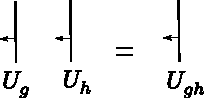
\includegraphics{groupmul.pdf}
    \end{align}
    \item 群の単位元には、自明な欠陥が対応。
    \begin{align}
      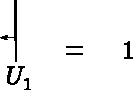
\includegraphics{groupidentity.pdf}
    \end{align}
    \item 逆元に対応するのは、向きを裏返したものである。
    \begin{align}
      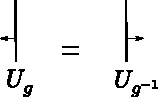
\includegraphics{groupinverse.pdf}
    \end{align}
  \end{enumerate}
  \item 局所演算子への作用
  \begin{align}
    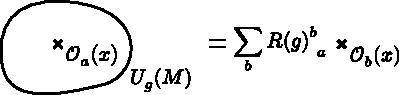
\includegraphics{EgWTid2.pdf}
  \end{align}
\end{itemize}

\section{一般化対称性}
これまで、普通の対称性がある種のトポロジカル欠陥という見方ができることが分かりました。逆に一般のトポロジカル欠陥は必ずしも対称性を表すものではありません。ここでのアイデアは、これを逆手にとって対称性の一般化を行うことです。
\begin{emphasize}
  一般のトポロジカル欠陥を\kyou{「一般化対称性」}と呼ぶ。
\end{emphasize}

まず、対称性はトポロジカル欠陥のうちで特殊なものでしたから、トポロジカル欠陥のことを一般化対称性と呼ぶのは妥当なことだと思います。大事なことはこの一般化対称性が普通の対称性と同じように場の理論の解析に使えるかということです。まず、トポロジカルという性質だけからWard-Takahashi恒等式に当たる恒等式を考えることができます。また導入の章で説明した例ですと、Hamiltonianと交換するというのはトポロジカルということです。この性質があると、普通の対称性でなかったとしても、ある場面では対称性と同様の使い方ができるということは、導入の章で説明したとおりです。ただし、一般化対称性をどのように使うかということに関しては、まだまだ研究の余地があり、現在も発展中です。

普通の対称性とは異なる一般化対称性には、ざっくり2つの方向性があります(もちろん両方の意味で一般化することも考えます)。
\begin{itemize}
  \item 普通の対称性は余次元1でしたが、これを余次元$p+1,\ p>0$にしたものは$p$形式対称性とか高次形式対称性と呼ばれます。
  \item 群構造が無いトポロジカル欠陥は「非可逆対称性」と呼ばれます。
\end{itemize}

非可逆対称性の名前の由来について、もう少しだけ説明します。まず、2つのトポロジカル欠陥を並べて置いたものはまたトポロジカル欠陥とみなすことができます。このような操作で新しいトポロジカル欠陥を作ることを\kyou{「フュージョン」}(fusion)といいます。これは対称性欠陥のまとめのところでも出てきました。普通の対称性の場合にはフュージョンは群の掛け算になります。また、自明なトポロジカル欠陥(何も置かない)ものは必ず存在します。自明なトポロジカル欠陥は任意のトポロジカル欠陥とフュージョンしても変化させないので、単位元の役割を果たします。つまり、群構造のうちで満たさない可能性があるのは逆元の存在です。考えているトポロジカル欠陥$A$に対して、フュージョンによって$A$を消すようなトポロジカル欠陥が存在しない場合に$A$や$A$を含むようなトポロジカル欠陥の集合を非可逆対称性と呼びます。

空間方向にのみ伸びているトポロジカル欠陥はHilbert空間に作用する演算子で、Hamiltonianと交換するものと思うことができます。このトポロジカル欠陥が非可逆対称性であることは、必ずしも\kyou{このHamiltonianと交換する演算子が逆演算子を持たないということではない}ということに注意してください。トポロジカル欠陥が非可逆というのは逆のトポロジカル欠陥が無いということです。演算子に逆があったとしても、それが非局所的で欠陥ですらないようなものの場合には、トポロジカル欠陥は非可逆といいます。

\end{document}